\documentclass{article}

\usepackage{tikz}
\usetikzlibrary{intersections}

\begin{document}
    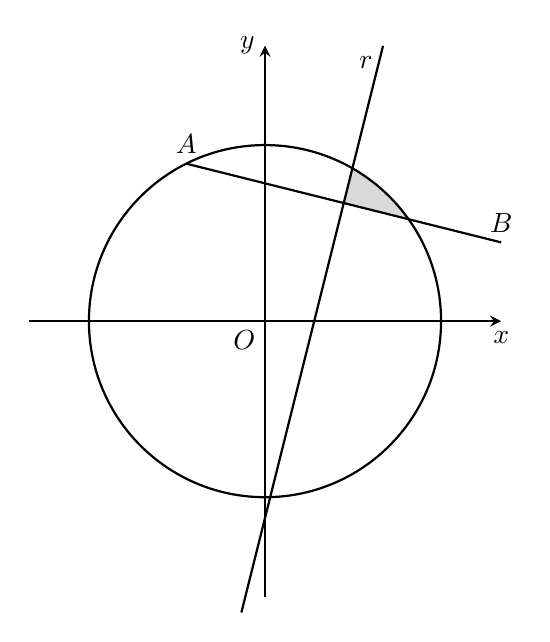
\begin{tikzpicture}

        \coordinate[label=below left:{$O$}] (O) at (0,0);
        \coordinate[label={$A$}] (A) at (-1,2);
        \coordinate[label={$B$}] (B) at (3,1);

        \path[name path=circunferencia] (O) circle ({sqrt(5)});
        \path[name path=retaAB] (A) -- (B);
        \path[domain=-0.3:1.5, samples=100, name path=retaR] plot (\x, 4*\x-2.5);
        
        % achar uma interseção de AB com circunferencia
        \path [name intersections={of=retaAB and circunferencia}];
        \coordinate (C) at (intersection-1);

        % achar uma interseção de r com circunferencia
        \path [name intersections={of=retaR and circunferencia}];
        \coordinate (D) at (intersection-2);

        % achar a interseção de r com AB
        \path [name intersections={of=retaR and retaAB}];
        \coordinate (M) at (intersection-1);

        %sombreado
        \begin{scope}
            \clip(0,0) circle ({sqrt(5)});
            \fill[draw=none, fill=gray!30] (M)--(B)--(1.5, {4*1.5-2.5});
        \end{scope}

        \draw[thick] (O) circle ({sqrt(5)});
        \draw[thick] (A) -- (B);
        \draw[thick, domain=-0.3:1.5, samples=100] plot (\x, 4*\x-2.5) node[below left]{$r$};
        
        \draw[->, thick, >=stealth] (-3,0) -- (3,0) node[below] {$x$};
        \draw[->, thick, >=stealth] (0,-3.5) -- (0,3.5) node[left] {$y$};
    \end{tikzpicture}
\end{document}